\chapter{本地开发环境与 IDE}
\label{chap:ide-tools}

\begin{introduction}
  \item 学习目标：为 CLion 与 VS Code 选好工具链，用同一份 CMake 工程完成构建和运行；用断点、单步与变量窗口核对一次函数调用。
  \item 建议学时：约半天，任选一套工具完成安装、运行和调试练习。
  \item 本卷边界：先用现成工程练本地工具，AstroNvim 配置按需选读。安装 Ubuntu、C++ 语法与 CMake 原理见卷一，远程编辑见卷一第 4 章的 SSH 一节。
\end{introduction}

第一次按顺序读准备工程一节，再从第~\ref{sec:ide-clion}、\ref{sec:ide-vscode}~节中任选一套工具。得到 \texttt{total = 75} 后，接着做第~\ref{sec:ide-debug}~节的断点练习。学完卷一的命令行基础后，也可以回来选读 AstroNvim。

\begingroup
\setlength{\emergencystretch}{3em}
\section{准备开发工具与练习工程}
\subsubsection{先分清编辑器、工具链和工程}

写代码需要编辑器，把代码变成程序需要编译器，暂停程序并查看变量需要调试器。
集成开发环境（Integrated Development Environment，IDE）把这些操作放进同一个窗口。
你们先前培训阶段可能使用过Dev C++这类较为基础的IDE，它对那些单文件程序来说可能够用，但是对我们下来的项目开发而言，是远远落后的。我们需要更专业的IDE来支持C++和CMake的开发。
CLion 面向 C/C++ 工程，集成了 CMake 和调试入口；Visual Studio Code（简称 VS Code）以编辑器为基础，通过扩展接入 C++ 和 CMake。
\textbf{VS Code 与 Visual Studio 是两个软件}，下载时看清名字。

工具链（Toolchain）包括编译器、构建工具和调试器等。CMake 读取工程描述，生成构建规则；编译器把源码编译成程序。
本章先把现成的小工程跑起来，但不会直接介绍工程内部详细的实现原理。代码不理解也没有关系。想提前学习的话：遇到看不懂的 C++ 写法，查卷一第 2 章；想弄清目标和构建规则，查卷一第 3 章。

\begin{center}
\begin{tabular}{p{0.19\textwidth}p{0.34\textwidth}p{0.34\textwidth}}
\toprule[1.5pt]
项目 & CLion & VS Code\\
\midrule[1pt]
C++ 支持 & 内置代码分析、CMake 与调试界面 & 安装 C/C++、CMake Tools 扩展\\
Windows 工具链 & 可使用随安装包提供的 MinGW & 另装工具链，本节采用 MSYS2 UCRT64\\
Ubuntu 工具链 & 使用系统 GCC、GDB 等 & 使用系统 GCC、GDB 等\\
打开工程 & 打开含 CMakeLists.txt 的文件夹 & File（文件）→ Open Folder（打开文件夹）\\
\bottomrule[1.5pt]
\end{tabular}
\end{center}

第一次任选一套软件，先把工程跑通并完成断点练习。对另外一个软件感兴趣时，再回来查另一套界面。\textbf{先完成所用系统的一条安装路线}，不要把 Windows、Ubuntu、WSL 的路径混着填。Ubuntu的安装可以等到你们安装完双系统后回看。
下面的 IDE 截图来自 Ubuntu 中的实际操作；在 Windows 中，同名工具窗口和工作流程基本相同。
图标位置会随版本、语言包、窗口宽度和扩展变化，找不到时先悬停看提示，再用菜单或动作搜索按名称查找。

\subsubsection{准备两套软件共用的练习工程}
教材附带 \texttt{examples/ide-demo} 目录。先复制一份作为自己的练习工程。
Windows 可放在 \texttt{C:/dev/ide-demo}，Ubuntu 可放在 \texttt{\textasciitilde/dev/ide-demo}。
也可以手动建立文件夹并创建下面两个文件。打开时选这一层目录，文件树顶层应直接出现 \texttt{CMakeLists.txt} 和 \texttt{main.cpp}。

\Needspace{23\baselineskip}
\begin{example}[计分器：预期输出 total = 75]
\texttt{main.cpp} 的完整内容如下：


\Needspace{19\baselineskip}
\lstinputlisting[language=C++,frame=single,numbers=left,showstringspaces=false]{examples/ide-demo/main.cpp}


\texttt{CMakeLists.txt} 的完整内容如下：


\Needspace{8\baselineskip}
\lstinputlisting[language=cmake,frame=single,numbers=left]{examples/ide-demo/CMakeLists.txt}


main 中先准备 score 与 bonus，调用 \texttt{add\_score}；函数把两个参数相加后返回，main 打印 total。CMakeLists.txt 指定工程语言、C++17 和源文件，\texttt{add\_executable} 建立运行目标。先记住：\texttt{ide\_demo} 是可执行目标名；\texttt{main.cpp} 是它的源文件；工程使用 C++17。
两套软件操作同一份源码时，分别使用自己的构建目录，避免不同编译器共用 CMake 缓存。若先用终端核对工程本身，可从本卷目录执行：


\Needspace{7\baselineskip}
\begin{tbash}
cmake -S examples/ide-demo -B /tmp/ide-demo-build -DCMAKE_BUILD_TYPE=Debug
cmake --build /tmp/ide-demo-build
/tmp/ide-demo-build/ide_demo
\end{tbash}


应输出 total = 75。已有同名构建目录且用过别的工具链时换一个新目录。
\end{example}

\section{用 CLion 开发}
\label{sec:ide-clion}
\subsubsection{安装 CLion：从安装包到工具链检查}

\paragraph*{Windows 安装步骤}
\begin{enumerate}
\item 从 JetBrains 官网下载与系统架构匹配的 CLion 安装包，运行安装程序，选择安装位置。
\item 在 Installation Options（安装选项）中按需勾选桌面快捷方式；Add launchers dir to the PATH 让终端能找到启动器，\textbf{不等于安装了编译器}；Open Folder as Project 增加资源管理器右键入口；文件关联决定双击 \texttt{.cpp} 等文件时用什么打开。这些选项不影响本节核心流程。
\item 完成安装后启动 CLion。首次启动可跳过导入旧设置，选择主题；若出现许可证页面，我们可以选用免费的教育许可。
\item 欢迎页的 New Project（新建项目）用于生成工程；Open（打开）用于打开已有工程；Get from VCS（从版本控制获取）用于克隆仓库；Customize（自定义）调整外观；Plugins（插件）管理扩展。中文界面可在插件页搜索 Chinese Language Pack，安装后按提示重启。
\item 打开工程后进入 File → Settings → Build, Execution, Deployment → Toolchains（文件→设置→构建、执行、部署→工具链）。选择 MinGW，Toolset 选 Bundled（捆绑），等待 C/C++ Compiler、Debugger 和 Build Tool 检测完成。若安装版本未附带工具链，先按官方 Windows 工具链教程安装，不能把编辑器目录当作编译器目录。
\end{enumerate}

\paragraph*{Ubuntu 安装步骤}
先准备本机编译工具，然后从 JetBrains 官网下载 Linux 版 CLion，或通过 JetBrains Toolbox 安装，或使用 Snap 安装。
\Needspace{8\baselineskip}
\begin{example}
安装并检查 Ubuntu 工具链：


\Needspace{9\baselineskip}
\begin{tbash}
sudo apt update
sudo apt install build-essential gdb cmake ninja-build
g++ --version
gdb --version
cmake --version
\end{tbash}


三个版本命令都应打印版本信息。若下载的是压缩包，在文件管理器中解压到自己的软件目录，进入解压目录的 \texttt{bin}，在终端执行 \texttt{./clion.sh} 启动。
然后在 Toolchains 中检查本机编译器路径；工具链可能叫 System（系统），也可能沿用默认名字 Default。CMake 可用捆绑版本或已安装的系统版本。
旧版的 GDB 路径也在这里设置；如果你用的是 CLion 2026.2 或更新版本，则到 Debugger → Debug Profiles（调试器→调试配置）选择 GDB，再核对顶部的 \texttt{Debug | GDB}。看到工具链里的 Debugger 项提示 deprecated，说明设置入口迁移了，不是编译器坏了。
\end{example}

\Needspace{7\baselineskip}
\begin{note}
安装与工具链参考：
\par{\footnotesize\url{https://www.jetbrains.com/help/clion/installation-guide.html}\par}
{\footnotesize\url{https://www.jetbrains.com/help/clion/quick-tutorial-on-configuring-clion-on-windows.html}\par}
Windows 的 MinGW 不能直接构建依赖 Ubuntu/ROS2 的工程；本节的跨平台小程序可以，后续 ROS2 实验应使用相应 Linux 环境。
\end{note}

\subsubsection{CLion 主界面：每一块负责什么}
\begin{figure}[H]
\centering
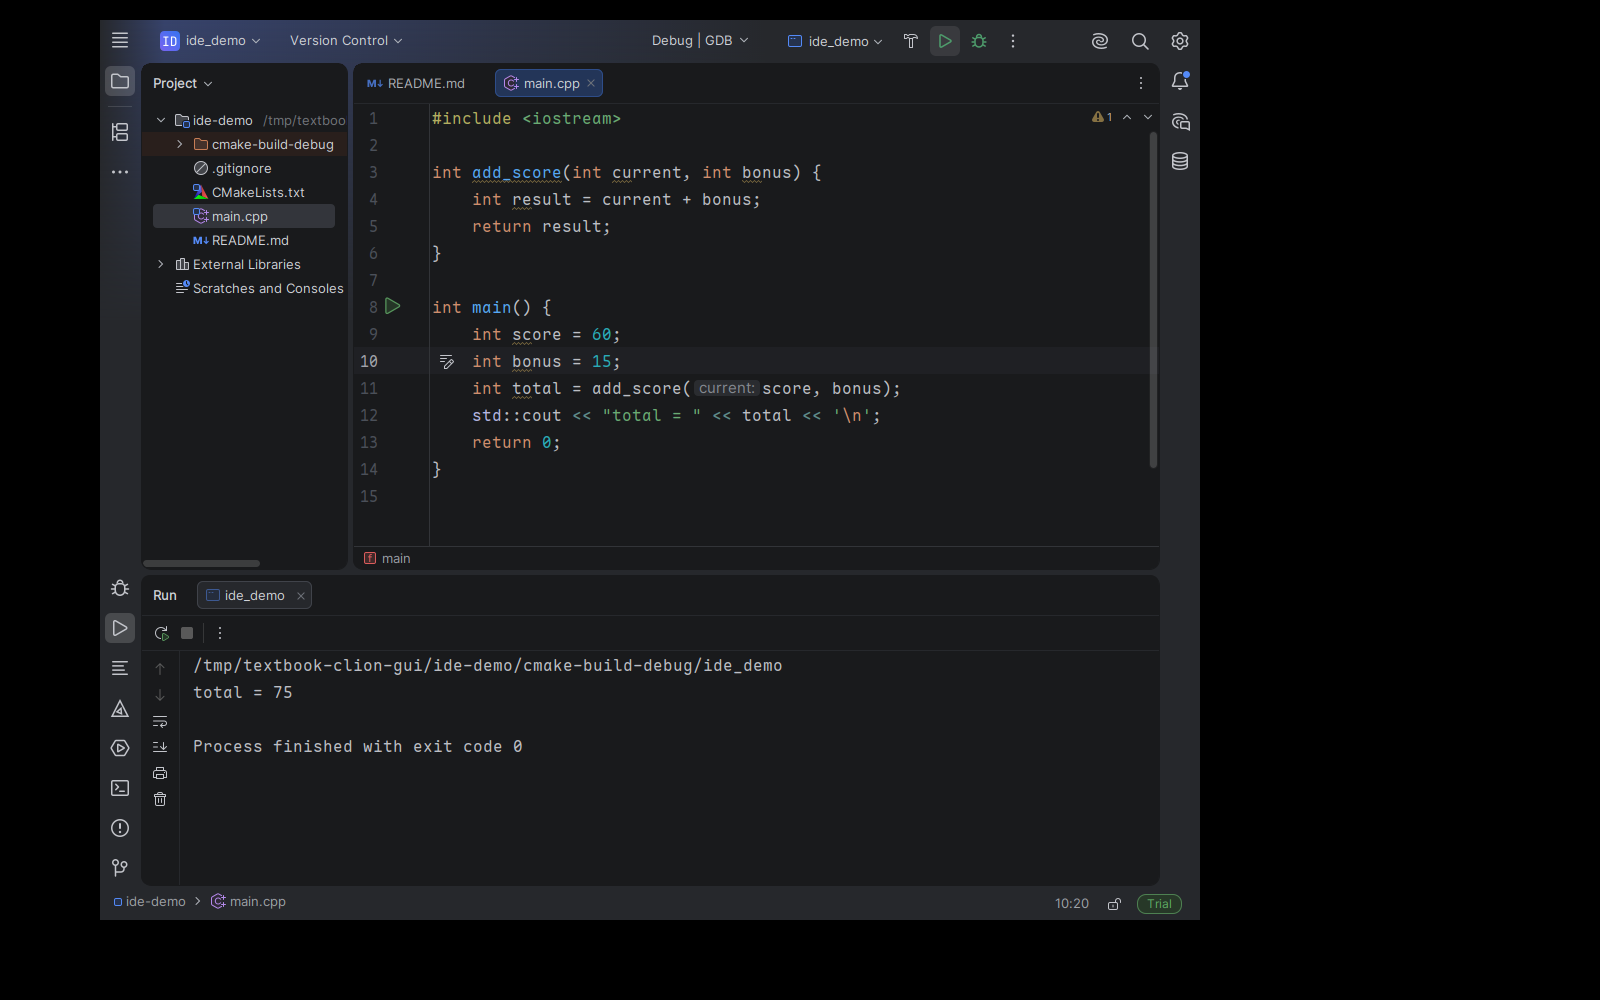
\includegraphics[trim=100bp 220bp 400bp 20bp,clip,width=0.9\textwidth]{ide/clion_run_revised.png}
\caption{CLion 2026.2.3 的界面：左侧工程目录、中央源码、顶部运行控件，底部输出 \texttt{total = 75} 并正常退出}
\label{fig:clion-overview}
\end{figure}

\textbf{先沿窗口边缘找入口，再看中央编辑区。} 下表按位置说明常用按钮；被折叠的工具窗口可从 View → Tool Windows（视图→工具窗口）重新打开。
\begingroup\small
\begin{longtable}{p{0.30\textwidth}p{0.60\textwidth}}
\toprule[1.5pt]
位置／按钮 & 点击后的功能与使用时机\\
\midrule[1pt]\endhead
左上角三横线主菜单 & 展开 File、Edit、View、Navigate、Code、Refactor、Build、Run、Tools、Git、Window、Help；打开项目、设置与退出从这里找。\\
顶部项目名下拉 & 切换或打开项目；先看名称，避免在别的工程中运行。\\
顶部 Git 分支名 & 查看、切换和新建分支；提交前核对分支。未启用 Git 时可能不显示。\\
顶部 Debug／Release 下拉 & 选择 CMake 配置；初学调试选 Debug。新版显示为 Debug | GDB，同时指出所选调试配置。构建参数和构建目录仍在 CMake 设置中检查。\\
顶部目标名下拉 & 选择运行目标；Edit Configurations（编辑配置）设置参数、环境变量、工作目录。\\
锤子 Build（构建） & 编译并链接所选目标，成功后生成程序；只构建不会执行程序。\\
三角 Run（运行） & 通常先构建再运行当前目标，在 Run 窗口看输出；普通运行不在断点暂停。\\
小虫 Debug（调试） & 带调试器启动目标，可在断点暂停并观察变量。\\
方块 Stop（停止） & 终止当前运行或调试进程；仅有活动进程时可用。\\
放大镜 Search Everywhere & 查找文件、符号和动作；连按两次 Shift 也能打开。\\
齿轮 Settings（设置） & 配置字体、快捷键、工具链等；注意区分全局设置与工程设置。\\
右侧铃铛 Notifications（通知） & 查看后台任务、更新和错误提示；读清内容再处理，通知不是编译结果的替代品。\\
顶部 AI／协作图标（若启用） & AI 入口提供代码辅助，Code With Me 等协作入口用于共享会话；本节的本机构建和调试不依赖它们。\\
窗口最小化／最大化／关闭 & 控制整个应用窗口；不同于关闭一个编辑标签或隐藏一个工具面板。\\
\bottomrule[1.5pt]
\end{longtable}\endgroup

\begingroup\small
\begin{longtable}{p{0.30\textwidth}p{0.60\textwidth}}
\toprule[1.5pt]
位置／按钮 & 点击后的功能与使用时机\\
\midrule[1pt]\endhead
左侧文件夹 Project（项目） & 展开目录；双击文件打开；右键目录→New 新建文件，右键文件→Refactor → Rename 重命名并更新引用。\\
左侧 Structure（结构） & 列出当前文件的函数、类等符号，点击可跳转。\\
编辑区顶部文件标签及叉号 & 切换／关闭文件；关闭标签不会删除磁盘文件。CLion 有自动保存机制，运行前仍可按 Ctrl+S 明确保存。\\
行号旁空白槽 & 单击添加／取消红色断点；右键断点可加条件。主函数旁的绿色三角可为相应目标运行或调试。\\
代码旁灯泡／波浪线 & 查看检查结果与建议修复；Alt+Enter 展开动作，先读说明再应用。\\
右侧滚动条标记 & 定位错误、警告和搜索命中；悬停查看提示，点击跳到相应位置。\\
CMake 工具窗口 & 查看配置与生成日志；Reload CMake Project（重新加载）重新读取构建描述，不等于编译。\\
Build（构建）窗口 & 查编译器、链接器输出；点击报错中的文件与行号跳转。\\
Run（运行）窗口 & 看程序输出与退出码；程序等待标准输入时，点击控制台输入。\\
Debug（调试）窗口 & 看调用栈、局部变量、监视表达式与单步控制，详见后面的调试表。\\
Terminal（终端） & 打开当前机器的 shell；Windows 默认终端不因此变成 Ubuntu。\\
Git／Commit 工具窗口 & 查看差异、选择提交文件、写提交说明；提交到本地与推送到远程是两步。\\
工具窗口的省略号／隐藏按钮 & 省略号管理该面板的选项与布局；隐藏只收起面板，不代表停止进程。\\
底部状态栏 & 行列号用于定位，UTF-8 是编码，LF/CRLF 是换行格式，缩进项控制空格／Tab。点击可调整，勿为消除提示随意改全文件。\\
\bottomrule[1.5pt]
\end{longtable}\endgroup

\subsubsection{在 CLion 中构建、运行和调试}
\begin{figure}[H]
\centering
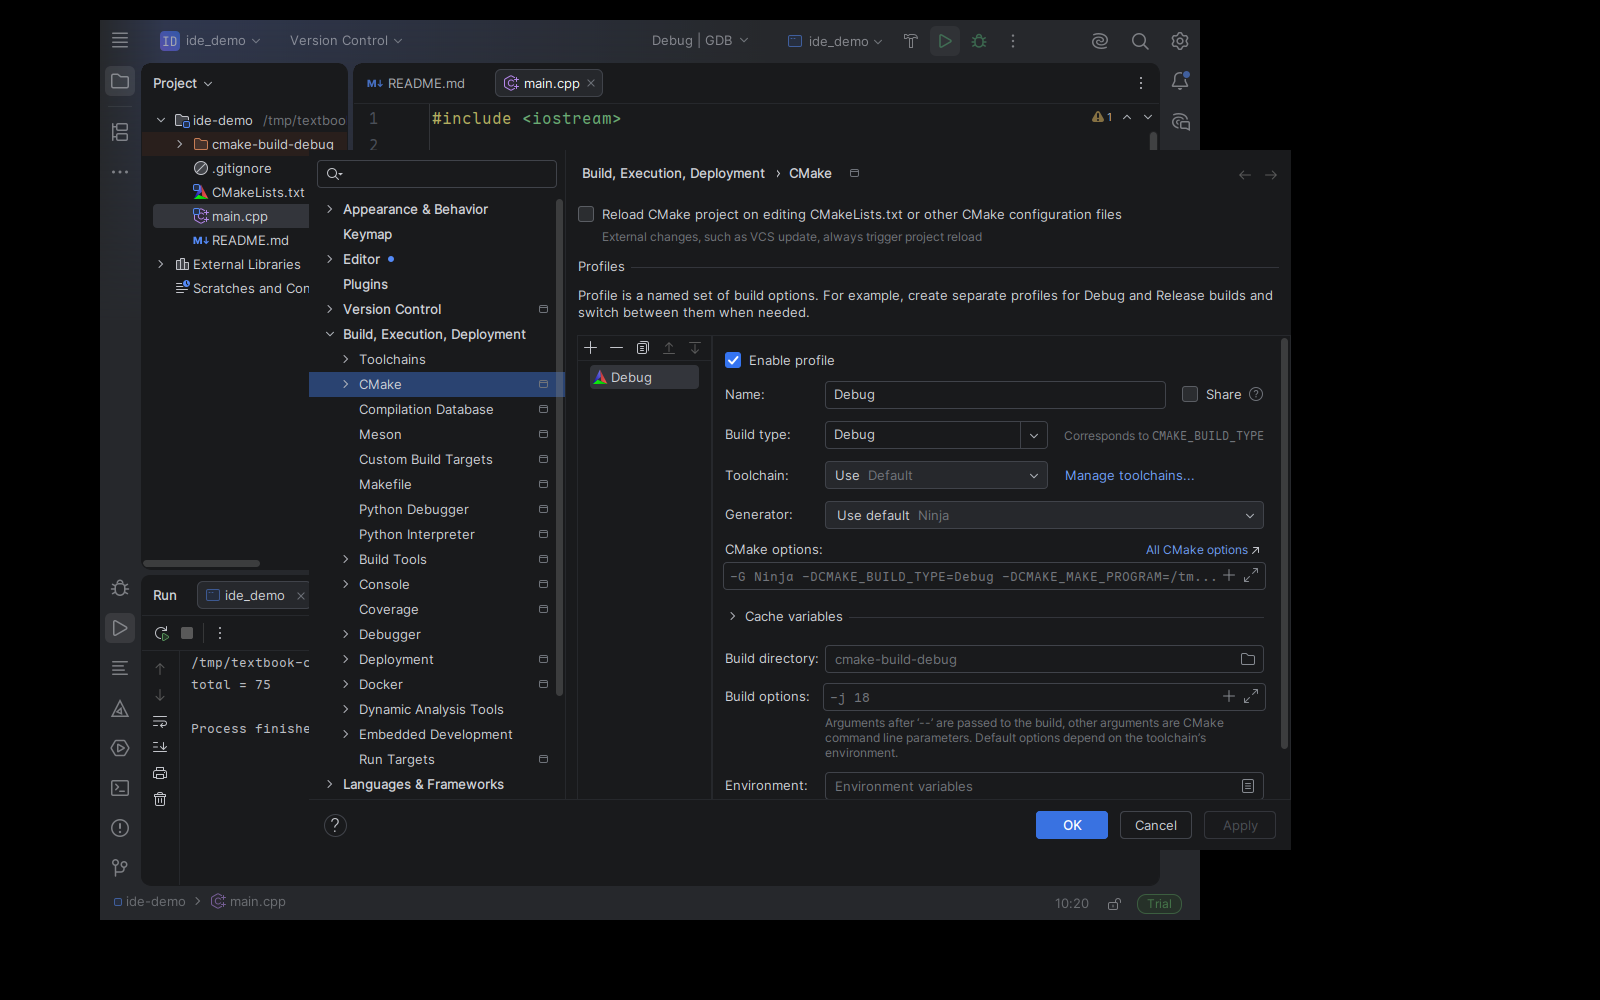
\includegraphics[trim=309bp 150bp 309bp 150bp,clip,width=0.9\textwidth]{ide/clion_cmake_revised.png}
\caption{CMake 设置：Debug 构建类型、默认本机工具链、Ninja 生成器，以及独立的 \texttt{cmake-build-debug} 目录}
\label{fig:clion-cmake}
\end{figure}
\Needspace{8\baselineskip}
\begin{example}
\begin{enumerate}
\item 用 Open 打开练习目录。若出现 CMake 向导，选 Debug、已检测成功的工具链和默认构建目录；等待配置完成。
\item 在顶部选择 \texttt{ide\_demo}，点锤子。Build 窗口应显示成功；再点绿色三角，Run 窗口应出现 \texttt{total = 75} 和退出码 0。
\item 打开 \texttt{main.cpp}，在第 11 行（调用 \texttt{add\_score}）左侧放断点，点小虫。程序暂停时该行\textbf{还没有执行}，所以此时不要读取尚未完成初始化的 \texttt{total}。
\item 在变量区确认 \texttt{score=60}、\texttt{bonus=15}。点 Step Into（步入）进入函数，查看形参 \texttt{current} 和 \texttt{bonus}；单步执行加法，再看 \texttt{result=75}。
\item 点 Step Out（步出）返回调用者，必要时再单步到下一条语句，确认 \texttt{total=75}；点 Resume（继续）直到输出并正常结束。
\end{enumerate}
\end{example}

如果打开工程后直接进入主界面，没有出现向导，我们就从 Settings → Build, Execution, Deployment → CMake 检查图中的配置。名字为 Debug 的配置还要核对 Build type 也确实是 Debug，然后等 CMake 配置完成，再点锤子构建。新版本可能把重新调试做成带回转箭头的小虫；程序还在运行时会先询问是否 Stop and Rerun（停止并重新运行），确认后才会启动新的进程。

运行参数位于目标下拉→Edit Configurations。本例不用参数，工作目录设为工程目录即可；以后程序使用相对路径读图片时，这个目录决定从哪里找文件。
设置里的 Toolchains 选择“用哪些工具”，CMake 配置选择“怎样构建”，运行配置选择“启动哪个程序、传什么参数”。三个入口各管一层。

\begin{exercise}\label{ex:ide-clion}
在 CLion 中将 \texttt{bonus} 改成 20，预测输出，再构建运行验证。在函数内部设置断点，记录执行加法前后的变量值，最后恢复为 15。
\end{exercise}

\Needspace{10\baselineskip}
\section{用 VS Code 开发}
\label{sec:ide-vscode}
\subsubsection{安装 VS Code 与 C++ 扩展}
\paragraph*{Windows 安装步骤}
\begin{enumerate}
\item 从 VS Code 官网下载对应架构的 Windows User Installer。运行后选择安装目录，按需勾选桌面快捷方式、右键“通过 Code 打开”与“添加到 PATH”。安装结束后重新打开终端，PATH 才会在新终端中生效。
\item 启动 VS Code，左侧点四个方块的 Extensions（扩展），搜索并核对发布者 Microsoft，安装 \textbf{C/C++}（\texttt{ms-vscode.cpptools}）和 \textbf{CMake Tools}（\texttt{ms-vscode.cmake-tools}）。二者分别提供 C++ 语言／调试支持和 CMake 工程操作。
\item 如需中文，安装 Microsoft 的 Chinese (Simplified) Language Pack，在命令面板中执行 Configure Display Language，选简体中文并重启。
\item 安装 C++ 编译工具。Windows 本节采用 MSYS2：从其官网安装到默认 \texttt{C:/msys64}，打开 \textbf{MSYS2 UCRT64} 终端，先执行 \texttt{pacman -Suy} 完整更新。若更新提示关闭终端，按提示退出所有 MSYS2 终端，重新打开 UCRT64 后再执行同一命令，直到没有待更新的软件包。然后运行下面的安装命令；遇到包组选择可回车使用默认项，再按提示确认安装。
\end{enumerate}


\Needspace{6\baselineskip}
\begin{tbash}
pacman -S --needed mingw-w64-ucrt-x86_64-toolchain
pacman -S --needed mingw-w64-ucrt-x86_64-cmake mingw-w64-ucrt-x86_64-ninja
\end{tbash}


在 Windows“编辑账户的环境变量”中编辑用户 Path，新增 \texttt{C:\textbackslash msys64\textbackslash ucrt64\textbackslash bin}（自定义安装则换成实际路径）。完全退出并重新打开 VS Code，在新 PowerShell 终端运行 \texttt{g++ --version}、\texttt{gdb --version}、\texttt{cmake --version}、\texttt{ninja --version}，应分别得到版本号。
若有多套工具链，用 \texttt{where.exe g++} 和 \texttt{where.exe gdb} 检查搜索顺序，随后在 CMake Tools 中选择 UCRT64 编译器作为 Kit。CMake Tools 会自动检测直接调试所用的调试器；若调试失败，再检查 GDB 是否来自同一套 UCRT64。

\paragraph*{Ubuntu 安装步骤}
从官网选择 Linux 的 \texttt{.deb} 安装包，架构与机器一致。在下载目录执行 \texttt{sudo apt install ./实际下载的文件名.deb}；这里要替换为真实文件名，不要原样照抄。
编译工具使用前面 Ubuntu 示例的安装命令。启动 VS Code 后同样安装 C/C++ 和 CMake Tools，工具链选系统 GCC。
\begin{note}
VS Code 本体及 C/C++ 扩展\textbf{不包含 C++ 编译器}。先确认版本命令能运行，再处理编辑器配置。
安装参考：\par{\footnotesize\url{https://code.visualstudio.com/docs/setup/windows}\par
\url{https://code.visualstudio.com/docs/setup/linux}\par}
Windows GCC 配置：\par{\footnotesize\url{https://code.visualstudio.com/docs/cpp/config-mingw}\par}
MSYS2 下载：\url{https://www.msys2.org/}。
\end{note}

\subsubsection{VS Code 主界面：活动栏、编辑器和底部面板}
\begin{figure}[H]
\centering
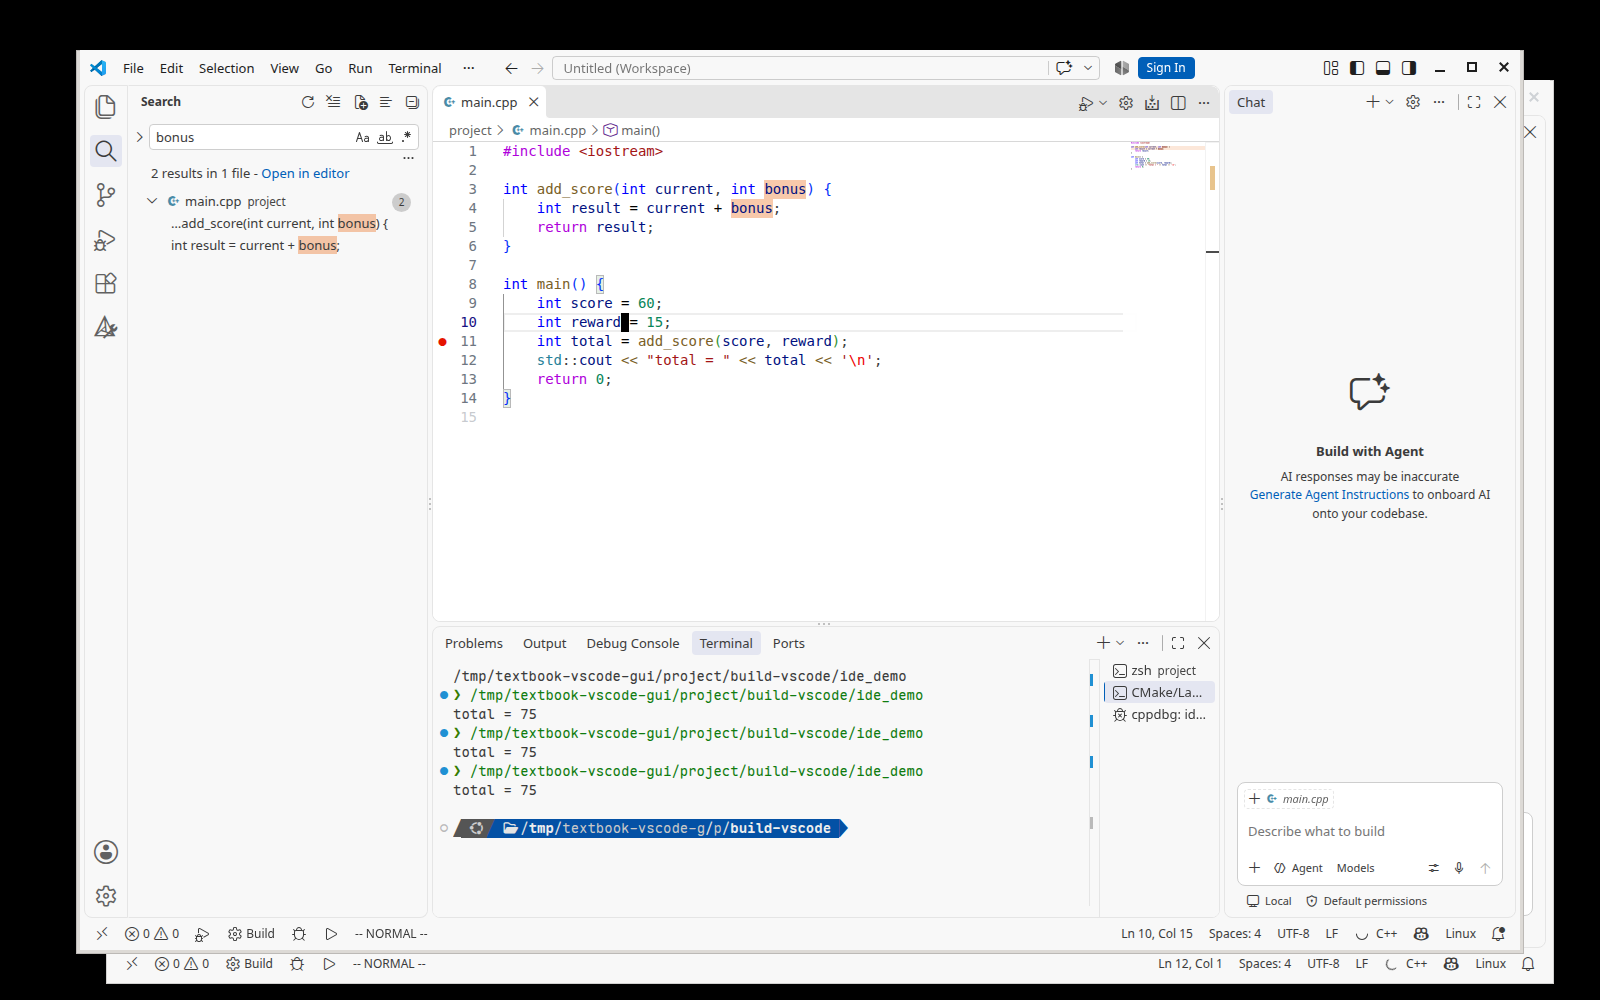
\includegraphics[trim=76bp 46bp 379bp 50bp,clip,width=0.9\textwidth]{ide/vscode_run_revised.png}
\caption{VS Code 1.139.1 的界面：搜索区、编辑区和集成终端；图中已经完成后面的重命名练习，\texttt{main} 中的变量改名为 \texttt{reward}，运行输出为 75}
\label{fig:vscode-overview}
\end{figure}

\begingroup\small
\begin{longtable}{p{0.30\textwidth}p{0.60\textwidth}}
\toprule[1.5pt]
位置／按钮 & 点击后的功能与使用时机\\
\midrule[1pt]\endhead
顶部 File／Edit／Selection & 文件菜单管理打开、保存；编辑菜单提供撤销、查找与替换；选择菜单提供多光标等选择操作。\\
顶部 View／Go／Run & 视图菜单显示面板与命令面板；转到菜单定位文件、行和定义；运行菜单管理调试。窄窗口可能折进省略号。\\
顶部 Terminal／Help & 终端菜单新建终端、运行任务；帮助菜单查看版本、文档和快捷键。\\
顶部搜索框／命令中心 & 快速打开文件、查找命令；Ctrl+P 搜索文件，Ctrl+Shift+P 打开命令面板。\\
左侧纸张 Explorer（资源管理器） & 显示文件树。悬停目录标题出现新建文件、新建文件夹、刷新和折叠全部按钮；双击文件固定标签，单击常为预览。\\
左侧放大镜 Search（搜索） & 跨文件搜索；展开替换框可批量替换。Aa 区分大小写，整词按钮限制完整单词，.* 启用正则表达式。\\
左侧分支 Source Control（源代码管理） & 查看差异；文件旁加号暂存，暂存区减号取消暂存，提交按钮创建本地提交。同步／推送会访问远程。\\
左侧三角加小虫 Run and Debug & 选择调试配置，查看变量、监视、调用堆栈和断点；单击大运行按钮可能要求先配置调试器。\\
左侧四方块 Extensions（扩展） & 搜索、安装、禁用或卸载扩展；齿轮管理某个扩展，核对发布者后再安装。\\
左侧 CMake 图标（安装扩展后） & 展开项目状态与项目大纲，选择工具链、配置、构建目标、启动目标并运行／调试。\\
左下角头像／齿轮 Manage & 头像用于账户相关功能；齿轮打开设置、快捷键、主题等。设置里区分 User（用户）和 Workspace（工作区）作用范围。\\
标题栏布局按钮 & 显示或隐藏主侧栏、底部面板、辅助侧栏等；隐藏侧栏不会关闭工程。\\
额外的活动栏图标 & Python、远程开发、AI 等扩展会增加入口；悬停看名称，用活动栏右键菜单管理显示项。\\
编辑标签、圆点和叉号 & 标签切换文件；圆点表示有未保存修改，Ctrl+S 保存；叉号关闭标签，不删除文件。\\
编辑区右上分栏／省略号 & 分栏可并排查看两个文件；省略号包含当前编辑器的更多动作。\\
编辑区右上三角及下拉 & 含义由语言与扩展决定，可能是运行当前文件；CMake 工程按后文的 CMake 命令运行整个目标。\\
面包屑／缩略图 & 面包屑显示文件路径与函数层级，点击定位；右侧缩略图帮助快速滚动长文件。\\
行号左侧与折叠箭头 & 点空白槽设断点；点折叠箭头收起代码块，不会删除代码。\\
Problems（问题） & 汇总诊断；点某条跳转到对应行，错误计数不等于本次构建一定失败，须结合构建日志判断。\\
Output（输出） & 看扩展日志，右侧下拉选择 CMake 等通道；通常不能在这里给程序输入。\\
Debug Console（调试控制台） & 看调试信息、求表达式值；C++ 程序的标准输入一般使用终端或外部控制台。\\
Terminal（终端） & 运行 shell 命令或与程序交互；加号新建终端，下拉选 PowerShell/Bash 等，分栏并排显示，垃圾桶结束该终端及其会话。\\
面板最大化／叉号 & 最大化扩大面板，叉号隐藏面板；隐藏终端面板不会自动结束里面的程序。\\
底部行列号、Spaces、UTF-8、CRLF/LF & 分别控制定位、缩进、编码和换行格式；C++ 表示当前语言模式，若误为 Plain Text，应改为 C++。\\
底部错误／警告、分支、远程标记 & 点计数打开问题；分支项处理版本控制；远程标记用于连接 WSL/SSH 等环境。先确认当前到底连在哪台机器。\\
\bottomrule[1.5pt]
\end{longtable}\endgroup

接下来用同一个计分器练习。配置或构建报错时，到 Output 的 CMake 通道看日志。程序启动后，再到 Terminal 核对实际输出。

\Needspace{10\baselineskip}
\subsubsection{在 VS Code 中运行同一个 CMake 工程}
\Needspace{8\baselineskip}
\begin{example}
\begin{enumerate}
\item File → Open Folder 打开练习目录。检查文件树顶层的两个文件。自己创建或已检查的教材工程可按提示信任；未知工程先在受限模式下检查内容。
\item 按 Ctrl+Shift+P 打开命令面板，输入 \texttt{CMake: Select a Kit}，选实际安装的 GCC：Windows 用 UCRT64，Ubuntu 用系统 GCC。若找不到，先运行 \texttt{CMake: Scan for Kits}。
\item 执行 \texttt{CMake: Select Variant}，选择 Debug；再执行 \texttt{CMake: Configure}。在 Output 中选 CMake 通道，确认配置、生成成功。
\item 执行 \texttt{CMake: Build}，等待成功，再执行 \texttt{CMake: Run Without Debugging}。若询问启动目标，选择 \texttt{ide\_demo}；终端应输出 \texttt{total = 75}。
\item 在第 11 行左侧点出红色断点，执行 \texttt{CMake: Debug}，观察程序停在该行。按后面表格单步并检查变量，再继续到退出。
\end{enumerate}
\end{example}

本例没有 CMake Presets，因而使用 Kit（工具链组合）与 Variant（构建类型）路线。
如果工作区启用了 Presets，命令可能变成 Select Configure Preset；先在工作区设置中将 \texttt{cmake.useCMakePresets} 设为 \texttt{never} 再做本例。
以后接手带 \texttt{CMakePresets.json} 的队内工程时，应使用工程提供的预设。
CMake Tools 的按钮可能在侧栏 Project Status，也可能在底部；\textbf{上述命令面板是布局变化时的备用入口}。
不过，输入动作名后先核对列表里的完整名字，再按回车：最近使用过的动作和相似名字可能排在前面。
例如 \texttt{CMake: Build} 是构建，\texttt{Append Build Directory to Current Workspace} 则是把构建目录加入工作区；名字里都有 Build，做的事情却不同。
若需要显式指定构建目录，可在工作区设置搜索 \texttt{cmake.buildDirectory}，使用 \texttt{\$\{workspaceFolder\}/build-vscode}。

\begin{note}
本例用 CMake Tools 直接启动调试，不要求手写 \texttt{launch.json}。
以后需要自定义时，\texttt{tasks.json} 描述任务，\texttt{launch.json} 描述如何启动调试，\texttt{c\_cpp\_properties.json} 配置代码分析；它们都不代替 \texttt{CMakeLists.txt}。
代码补全无红线只能说明分析器接受配置，不能证明程序已经编译成功。
\end{note}

\begin{exercise}\label{ex:ide-vscode}
用 VS Code 打开同一练习工程，搜索 \texttt{bonus}，跳转到定义，再将它重命名为 \texttt{reward}（使用 Rename Symbol／重命名符号，而非无差别全文替换）。保存、构建并运行，确认输出仍为 75；最后撤销并保存。
\end{exercise}

\section{单步调试与常见问题}
\label{sec:ide-debug}
\subsubsection{调试工具栏：不要只记小虫和三角}
\begin{figure}[H]
\centering
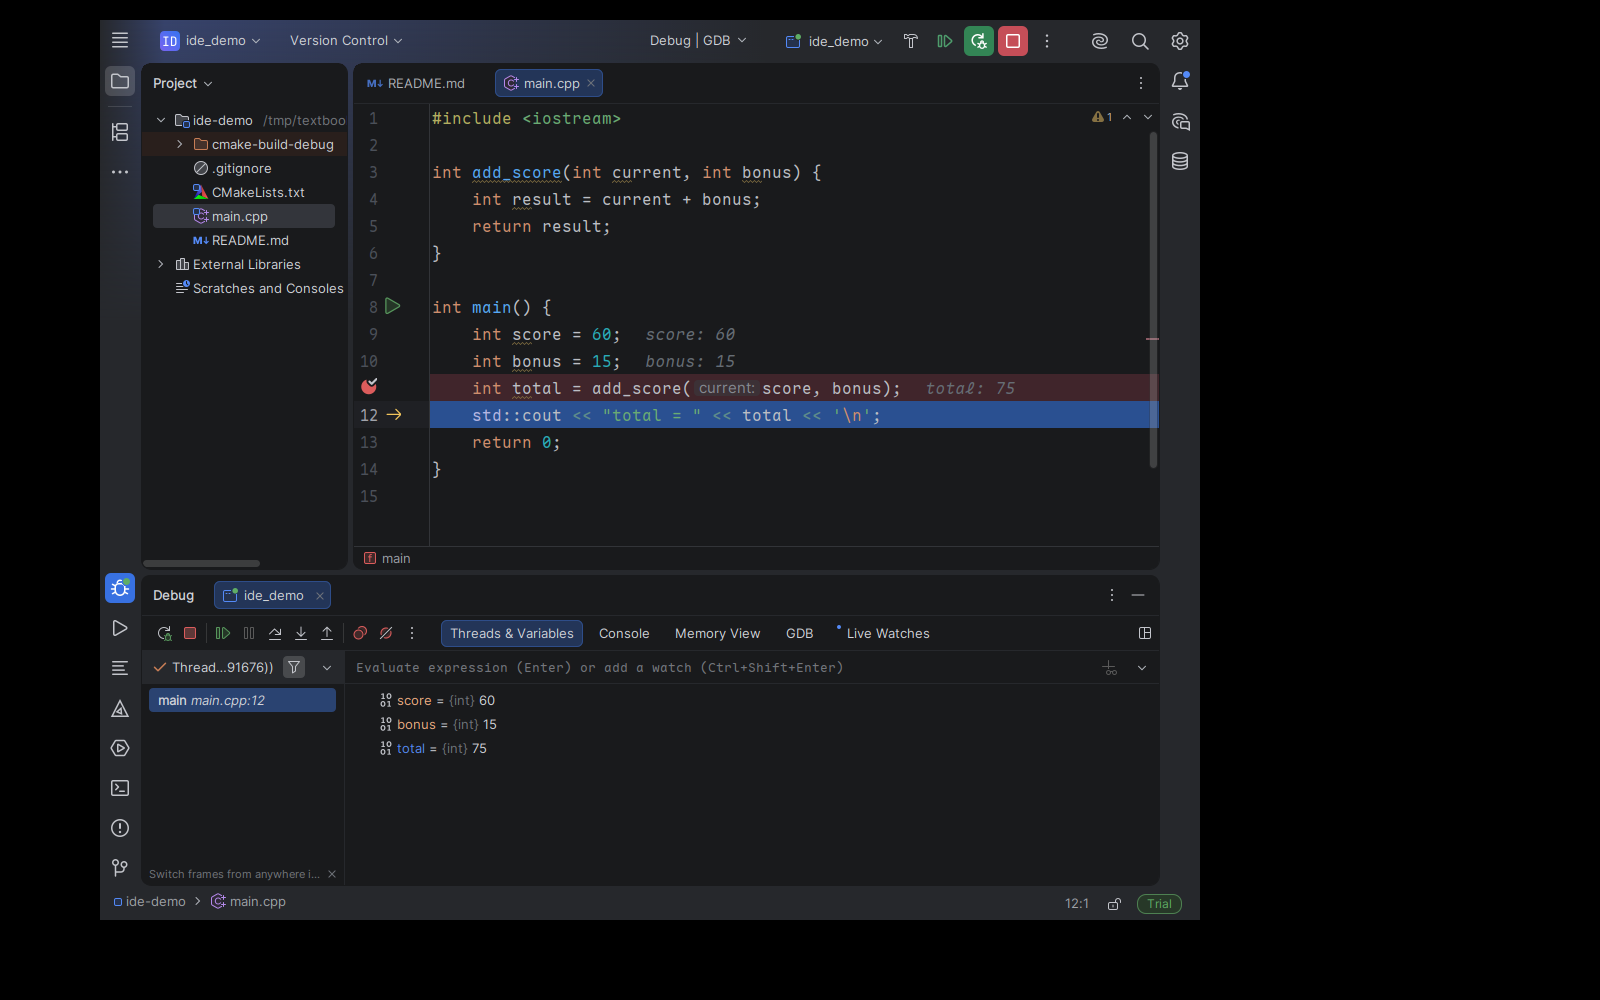
\includegraphics[trim=100bp 220bp 400bp 20bp,clip,width=0.9\textwidth]{ide/clion_debug_revised.png}
\caption{CLion 实际单步后停在第 12 行：第 11 行赋值已完成，变量区显示 \texttt{score=60}、\texttt{bonus=15}、\texttt{total=75}；左侧为调用栈，底部为单步按钮}
\label{fig:clion-debug}
\end{figure}
调试（Debugging）的目标是观察程序如何执行。断点让程序在某行执行前暂停，单步决定下一次停在哪里。
以下快捷键为 Windows/Linux 常见默认键位；若换过 Keymap，以按钮悬停提示为准。
\begingroup\small
\begin{longtable}{p{0.28\textwidth}p{0.14\textwidth}p{0.16\textwidth}p{0.31\textwidth}}
\toprule[1.5pt]
按钮／功能 & CLion & VS Code & 使用时机\\
\midrule[1pt]\endhead
Continue／Resume 继续（三角） & F9 & F5 & 跑到下一断点或程序结束。\\
Pause 暂停（双竖线） & 看工具栏 & F6 & 运行中请求暂停，排查卡在哪里。\\
Step Over 步过（弯箭头） & F8 & F10 & 执行当前行，函数调用整体完成。\\
Step Into 步入（向下箭头） & F7 & F11 & 进入当前行调用的函数内部。\\
Step Out 步出（向上箭头） & Shift+F8 & Shift+F11 & 执行到当前函数返回调用者。\\
Restart／Rerun 重新开始（回转箭头） & 看工具栏 & Ctrl+Shift+F5 & 重新启动进程，不是把时间倒回上一行。\\
Stop 停止（方块） & Ctrl+F2 & Shift+F5 & 结束当前调试会话／启动的程序。\\
Toggle Breakpoint 切换断点 & Ctrl+F8 & F9 & 在当前行添加或取消断点。\\
\bottomrule[1.5pt]
\end{longtable}\endgroup

\begin{figure}[H]
\centering
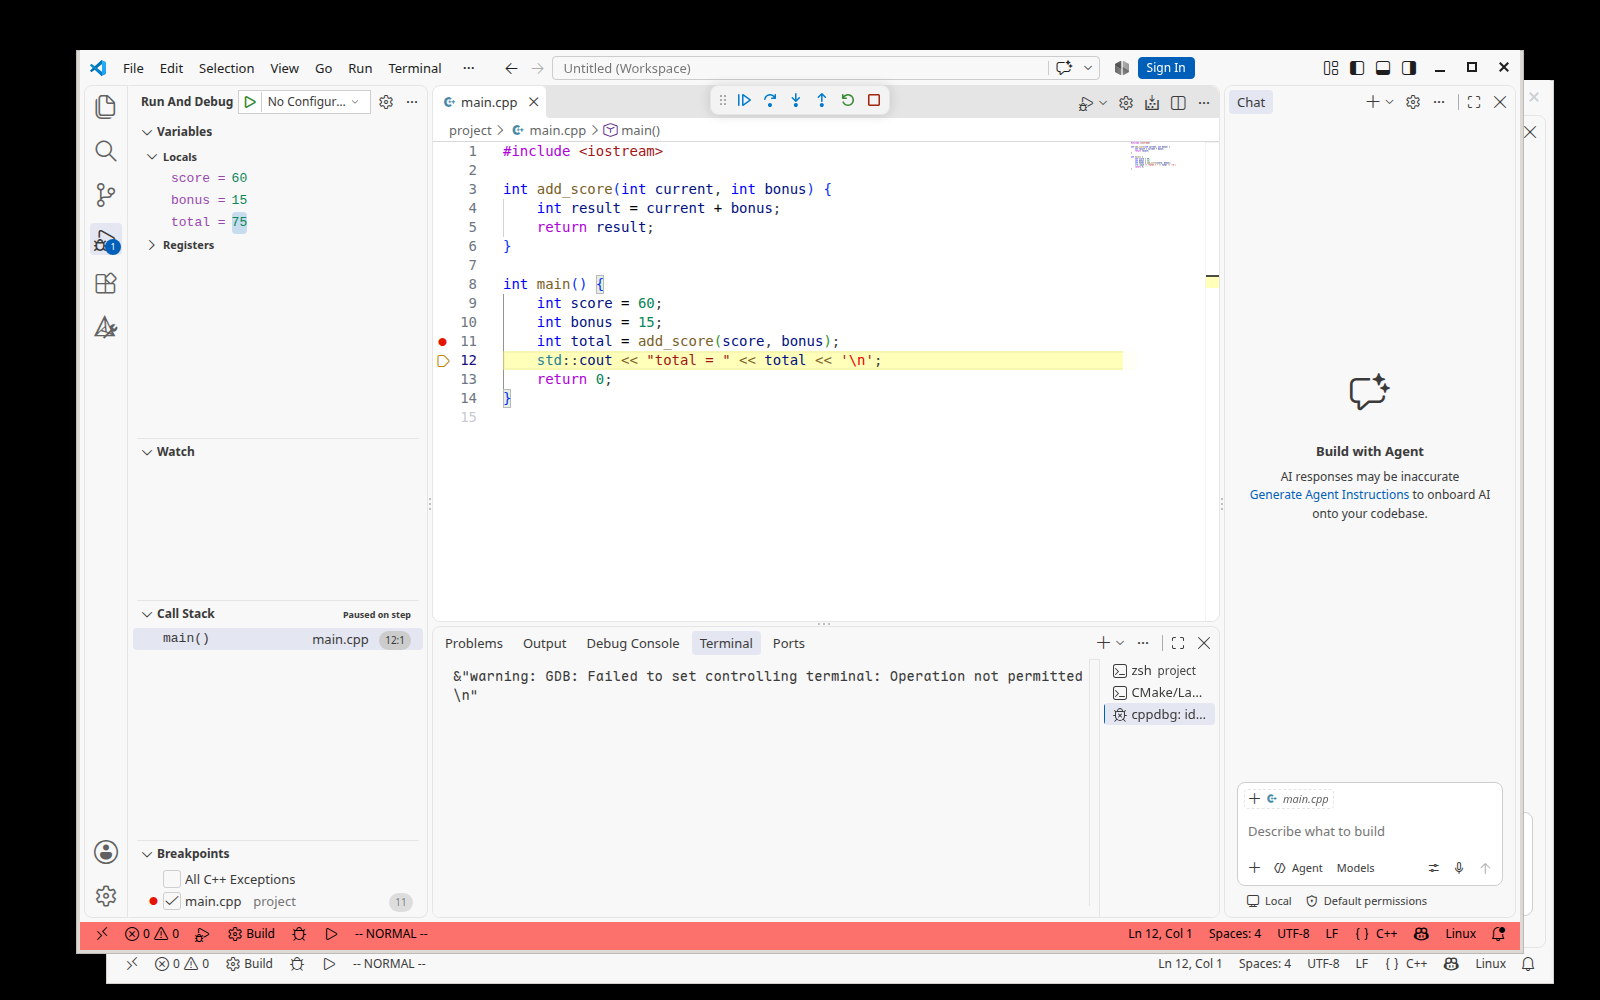
\includegraphics[trim=76bp 375bp 379bp 50bp,clip,width=0.9\textwidth]{ide/vscode_debug_revised.png}
\caption{VsCode 中的实际单步结果：执行第 11 行后停在第 12 行，左侧 \texttt{total = 75}；顶部是调试工具栏}
\label{fig:vscode-debug}
\end{figure}
\textbf{变量（Variables）}显示当前栈帧的局部变量；\textbf{监视（Watches/Watch）}可以添加 \texttt{score + bonus} 等表达式；
\textbf{调用栈（Frames/Call Stack）}显示函数调用关系，点击不同帧会切换变量作用域；\textbf{断点列表（Breakpoints）}集中启用、禁用或移除断点。
表达式必须在当前作用域有效：进入 \texttt{add\_score} 后看形参 \texttt{current}，想查看 \texttt{main} 的 \texttt{score} 则切回它的栈帧。
在暂停状态下查看简单表达式即可；会修改变量或调用函数的表达式可能改变被调试程序。

\begin{conclusion}
\begin{itemize}
\item 保存只把修改写到磁盘；配置读取 CMake 规则；构建生成程序；运行启动程序；调试带着调试器启动程序。
\item Run 不停在断点，Debug 才会；断点高亮行尚未执行，变量也必须已初始化才有可解释的值。
\item 工具链、构建配置、运行配置分开检查；界面布局变了就按动作名搜索，不凭图标颜色猜功能。
\end{itemize}
\end{conclusion}

\subsubsection{常见问题与排查顺序}
\begingroup\small
\begin{longtable}{p{0.29\textwidth}p{0.61\textwidth}}
\toprule[1.5pt]
现象 & 先检查什么\\
\midrule[1pt]\endhead
找不到编译器或 CMake & 在当前环境的终端查版本和路径；安装后重启 IDE。CLion 检查 Toolchains，VS Code 检查 Kit，不能只安装扩展。\\
运行按钮灰色／没有目标 & 是否打开了含 CMakeLists.txt 的目录？CMake 配置是否成功？该文件中是否创建了可执行目标？\\
修改了代码但输出不变 & 保存文件，检查当前工程、构建目录和启动目标，再构建运行，避免运行另一份旧程序。\\
断点空心／不停／变量被优化 & 使用 Debug 构建并启动调试；确认正在运行刚构建的程序，断点所在代码确实会执行。\\
更换工具链后 CMake 报缓存冲突 & 为新工具链换一个构建目录并重新配置；不要让 MSVC、MinGW、Linux 共用缓存。\\
终端有输出却不能输入 & 确认是 Terminal/Run 控制台，且程序还活着并在读输入；Output 只是日志。本例输出后立即退出。\\
编辑器红线与构建结果不一致 & 检查 C++ 扩展的编译器路径、标准与 CMake 配置提供者，再查看真实构建日志。\\
Windows 能跑，Ubuntu 找不到文件 & 检查路径大小写、斜杠、工作目录和系统依赖；不要复制 Windows 可执行文件到 Ubuntu 当作本机程序。\\
\bottomrule[1.5pt]
\end{longtable}\endgroup

\begin{exercise}\label{ex:ide-setup}
按所选工具完成练习~\ref{ex:ide-clion} 或~\ref{ex:ide-vscode}，再记录当前系统、编译器路径、Debug 构建目录和一次运行的退出码。在界面中指出终端、构建日志、运行输出和变量窗口。以后换工具时，用同一份记录对照。
\end{exercise}

\begin{exercise}\label{ex:ide-debug}
在第 11 行的函数调用前暂停，先预测步入后最先能看到的参数和值。步入后查看当前栈帧，再步出并单步到第 12 行，核对 \texttt{total}。如果断点未命中，说明会怎样检查构建类型和正在调试的目标。
\end{exercise}

\begin{note}
界面与操作核对资料：
\par\footnotesize
\url{https://www.jetbrains.com/help/clion/guided-tour-around-the-user-interface.html}\par
\url{https://www.jetbrains.com/help/clion/debugging-code.html}\par
\url{https://www.jetbrains.com/help/clion/configuring-debugger-options.html}\par
\url{https://code.visualstudio.com/docs/getstarted/userinterface}\par
\url{https://code.visualstudio.com/docs/cpp/cmake-linux}\par
\url{https://code.visualstudio.com/docs/debugtest/debugging}
\end{note}
\endgroup

\section{终端开发环境：AstroNvim*}
\label{sec:astronvim-customize}

Vim 本身有语法高亮与基础补全，但插件组合需要配置。Neovim（nvim）是 vim 的现代化分支，而 AstroNvim 是一套开箱即用的 Neovim 配置——装完就有文件树、模糊搜索、代码补全和漂亮的界面，毛坯房直接变精装，终端里也能有接近 IDE 的体验。

\textbf{安装新版 Neovim}

AstroNvim 需要较新版本的 Neovim，而 Ubuntu 22.04 仓库自带的版本太老，因此先核对官方要求再安装。下面仅用于 \texttt{x86\_64}，如果是在 Nvidia Orin NX 等 ARM 机器安装需要换用 arm64 架构包：

\Needspace{8\baselineskip}
\begin{example}
下载并解压 Neovim 到 \texttt{/opt}，顺手装上两个依赖（ripgrep 用于全局搜索，gcc 用于编译语法高亮组件）：


\Needspace{8\baselineskip}
\begin{tbash}
curl -fLO https://github.com/neovim/neovim/releases/latest/download/nvim-linux-x86_64.tar.gz
sudo tar -C /opt -xzf nvim-linux-x86_64.tar.gz
sudo apt install ripgrep gcc
\end{tbash}


然后把刚刚解压出的 bin 目录放到 PATH 前面，这样 Shell 会优先找到新版 Neovim。下面的设置只对当前会话生效；想长期使用，可以把这一行写入自己的 Bash 或 zsh 配置，方法见卷一第 1 章《Shell 脚本与环境变量》一节：


\Needspace{5\baselineskip}
\begin{tbash}
export PATH=/opt/nvim-linux-x86_64/bin:$PATH
\end{tbash}


生效后执行 \texttt{command -v nvim} 与 \texttt{nvim --version}，确认找到的是新安装的程序且版本满足要求；若旧版抢先被找到，把新目录放到 PATH 前面。
\end{example}

\textbf{安装 AstroNvim}

先用独立配置试用 AstroNvim。这里用 \texttt{NVIM\_APPNAME} 让 Neovim 把本次的配置、数据和缓存放到名为 \texttt{astronvim-training} 的目录下。需要 Git，已有同名练习目录时先换一个名字，并同步修改下面两处。
\href{https://docs.astronvim.com/reference/alt_install/}{官方独立安装说明}还给出了设置常用启动命令的方法。

\begin{example}[用独立配置打开练习工程]
在 Ubuntu 终端中执行以下命令，最后一行在复制好的 \path{ide-demo} 根目录运行。

\begin{tbash}
git clone --depth 1 https://github.com/AstroNvim/template ~/.config/astronvim-training
NVIM_APPNAME=astronvim-training nvim .
\end{tbash}

首次启动会下载插件。等待安装完成，再用空格键打开快捷键菜单，试着搜索 \texttt{main.cpp}。运行普通的 \texttt{nvim} 时会使用你平时的配置。
\end{example}

\begin{figure}[H]
    \centering
    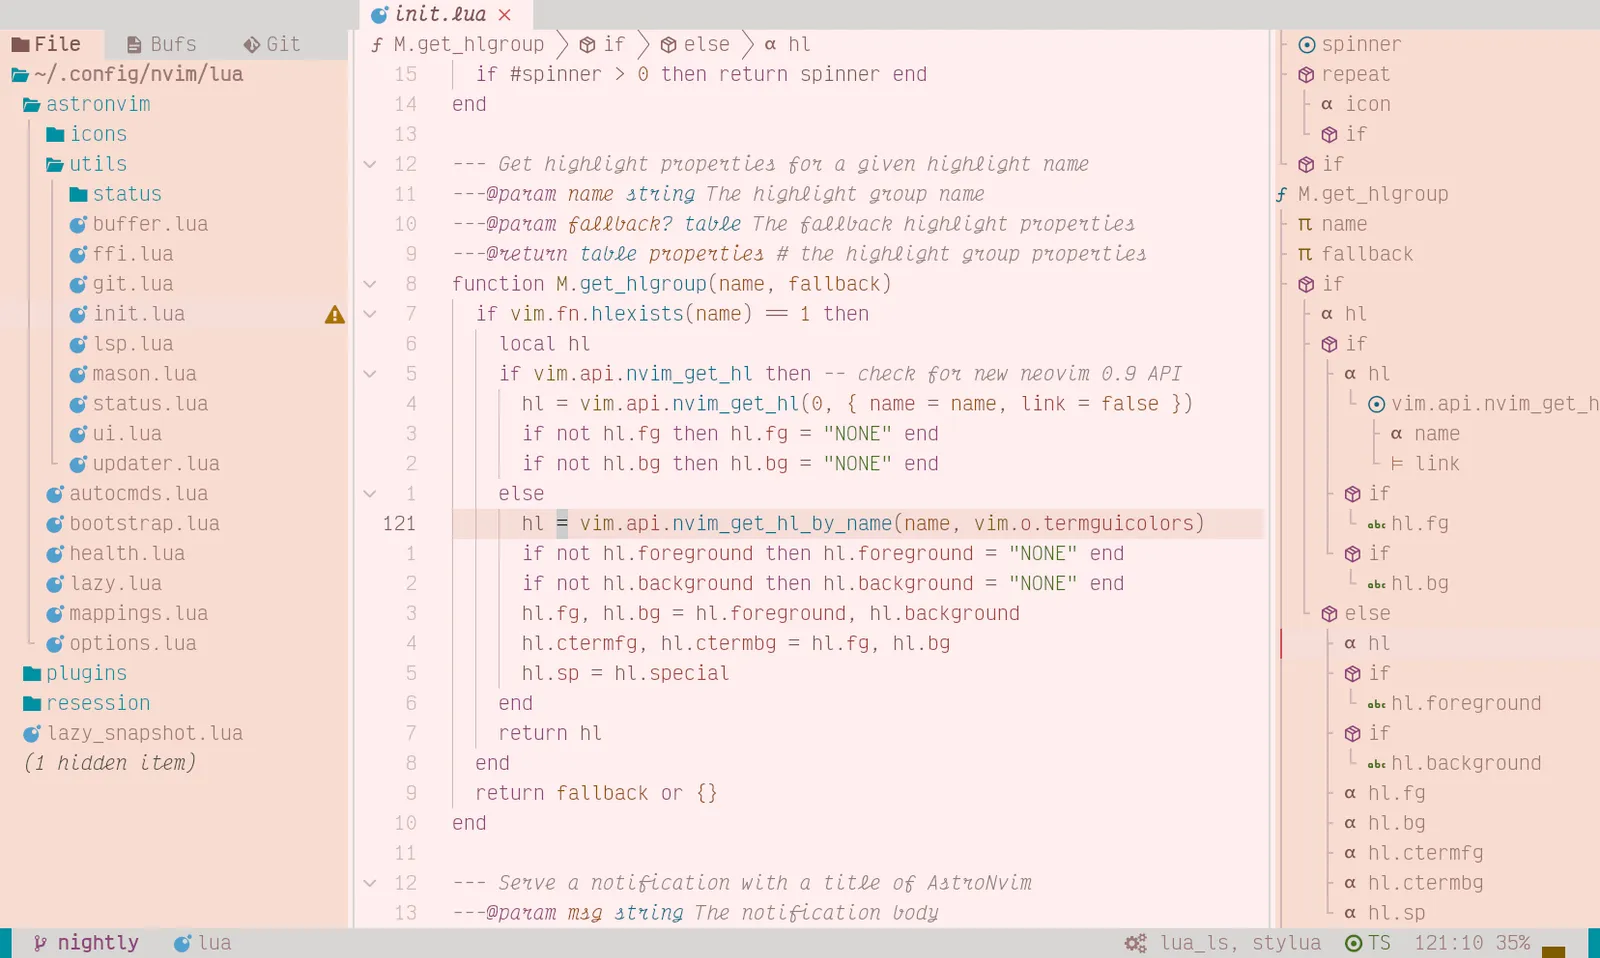
\includegraphics[width=0.8\textwidth]{ide/astronvim_welcome.png}
    \caption{AstroNvim 界面}
    \label{fig:astronvim}
\end{figure}

\textbf{上手要点}

\begin{itemize}
\item Leader 键是空格：按下 \texttt{<Space>} 稍等片刻会弹出快捷键菜单，忘了按键组合也不用背，跟着菜单按就行；
\item \texttt{<Space>ff} 模糊搜索并打开文件，\texttt{<Space>fw} 在整个项目中搜索文字（依赖 ripgrep）；
\item 在 \texttt{:Mason} 中查找并安装 \texttt{clangd}，打开 \texttt{main.cpp} 后用 \texttt{:checkhealth vim.lsp} 核对语言服务器已连接，再试补全和跳转。
\end{itemize}

\begin{note}
界面中的图标和 zsh 的 p10k 主题一样依赖 Nerd Font，装过 MesloLGS NF 的话直接通用（见卷一附录《zsh 与终端美化》）。更多用法见官方文档：\url{https://docs.astronvim.com/}
\end{note}

\begin{exercise}\label{ex:v0-astronvim}
完成 AstroNvim 的安装，用 \texttt{<Space>ff} 打开任意一个文本文件，再用 \texttt{<Space>fw} 在某个项目目录中搜索一个关键词，体验模糊搜索。
\end{exercise}

\section{本章小结}
CLion 和 VS Code 用的是同一条工作流：先确认当前系统和工具链，再打开含 \texttt{CMakeLists.txt} 的目录、配置目标、构建并运行。程序结果与预期不同时，用 Debug 构建停在断点，沿调用栈和变量值逐步核对。换 IDE 时，可以先找这些动作的入口，再熟悉界面布局。习惯终端的同学也可以用 AstroNvim 编辑与导航，并在终端运行 CMake 命令。下一章仍会用到这条工作流：让 AI 协助改代码之后，你要能亲自构建、调试并验证结果。

\begin{problemset}
\item \label{prob:v0-ide-1} （基础）分别说明 CLion 的锤子、绿色三角、小虫按钮的作用，以及 VS Code 的 Explorer、Extensions、Terminal、Output 各负责什么。为什么装好 VS Code 的 C/C++ 扩展后仍可能无法编译？
\item \label{prob:v0-ide-2} （提高）同一份源码先用 Windows 的 MinGW 构建，再用 Ubuntu 中的 GCC 打开。可以沿用同一个 CMake 构建目录吗？如果改了源码却仍看到旧输出，应依次核对什么？
\item \label{prob:v0-ide-3} （实践）在练习副本把 bonus 改为 25，先预测输出，再用一套 IDE 的 Debug 配置构建并验证。在第 11 行步入函数，记录两个参数；回到调用者后观察 total。提交实际构建目录与对应输出。
\end{problemset}

\section{本章验收}
\begin{enumerate}
\item 任选 CLion 或 VS Code 打开教学工程，指出菜单、文件树、编辑区、构建入口、运行入口、调试入口、终端和状态栏，并运行得到 \texttt{total = 75}。
\item 在所选工具中现场断点调试：在函数调用处暂停，演示步入、步过、步出、继续；指出当前栈帧与变量值，并解释为什么暂停行的赋值尚未生效。
\end{enumerate}

进阶练习时，再换另一套工具跑同一份源码，比较工具链选择、独立构建目录和调试入口。
